\subsection{Dataset Collection}

\noindent Our dataset acquisition process involved the following steps:


\subsubsection{Public Datasets}
A significant part of our extensive dataset was thoughtfully put together from openly accessible collections of deepfake and authentic images. We carefully chose these datasets to make our deepfake detection model more diverse and applicable. This approach helps us ensure a strong and thorough training and testing process by making the most of these available resources.

Here's the breakdown of our dataset:
\begin{itemize}
    \item \textbf{Trained:} 70,000 samples
    \item \textbf{Tested:} 5,000 samples
    \item \textbf{Validation:} 15,000 samples
\end{itemize}
Our dataset contains data from well-known public sources, and each of these sources has a specific role in making our deepfake detection system better :

\begin{enumerate}
    \item \textbf{DFDC (DeepFake Detection Challenge) Dataset:} The DFDC dataset offers an invaluable benchmark for detecting deepfake manipulations across a wide spectrum of scenarios and visual contexts. Its meticulous curation and large-scale inclusion of deepfake and real videos enable us to train our model on highly realistic and challenging instances.
    \item \textbf{Multi-Modal-CelebA-HQ:}The Multi-Modal-CelebA-HQ stands as an extensive face image dataset featuring 30,000 high-resolution facial images curated from the CelebA dataset through the CelebA-HQ process. Each image within this dataset is accompanied by a high-quality segmentation mask, a sketch, descriptive text, and an image with a transparent background.

    \item \textbf{CelebA Dataset:} By incorporating the CelebA dataset, a prominent repository of celebrity faces in diverse poses and expressions, we bolster our model's capacity to handle variations in lighting conditions, facial orientations, and natural facial expressions – all critical aspects in detecting nuanced manipulations.

    \item \textbf{CASIA WebFace Dataset:} With the CASIA WebFace dataset, we tap into a wealth of real facial images sourced from the internet, exposing our model to a plethora of natural variations in appearance, pose, and lighting conditions. This exposure fortifies our model's ability to discern between real and manipulated facial features in an ever-evolving digital landscape.
\end{enumerate}


\subsubsection{Video Conversion}
To include videos in our dataset, we first converted them into individual frames (images) to facilitate compatibility with the vision transformer architecture. This step involved extracting frames at a consistent frame rate from each video, resulting in a sequence of images for each video.
\begin{figure}[htbp]
    \centering
    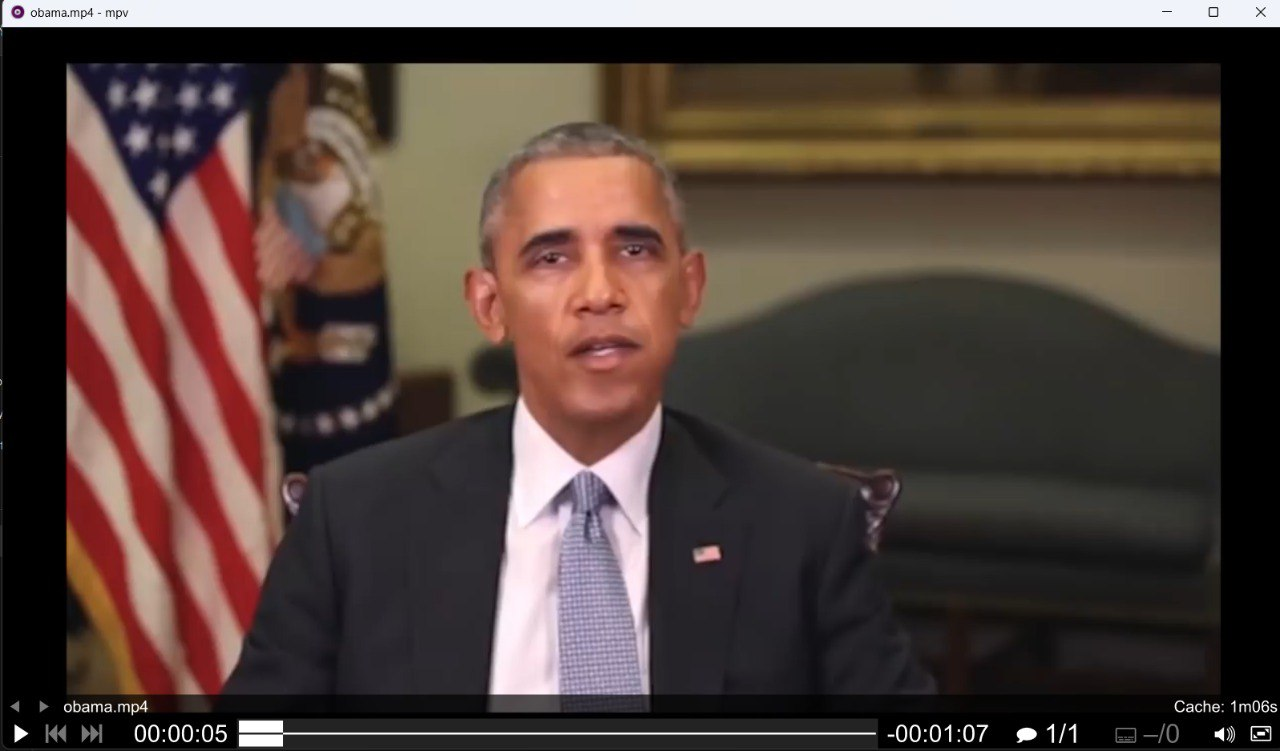
\includegraphics[width= 5in ]{img/framesExtracted.jpg}
    \caption{\textit{Video Sample}}
\end{figure}
\begin{figure}[ht]
    \centering
    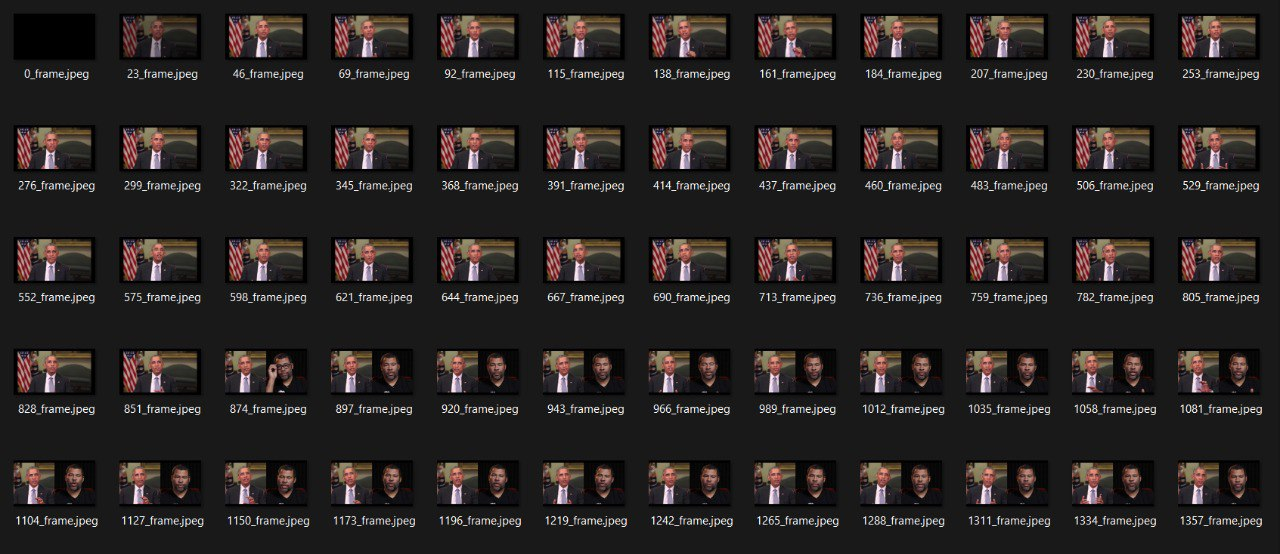
\includegraphics[width= 5in ]{img/frames.jpg}
    \caption{\textit{Frames Extracted from video}}
\end{figure}

\subsubsection{Frame Selection}
To avoid redundancy and maintain dataset balance, we carefully selected frames from videos to represent various stages of manipulation, expressions, poses, and lighting conditions.

\begin{figure}[htbp]
    \centering
    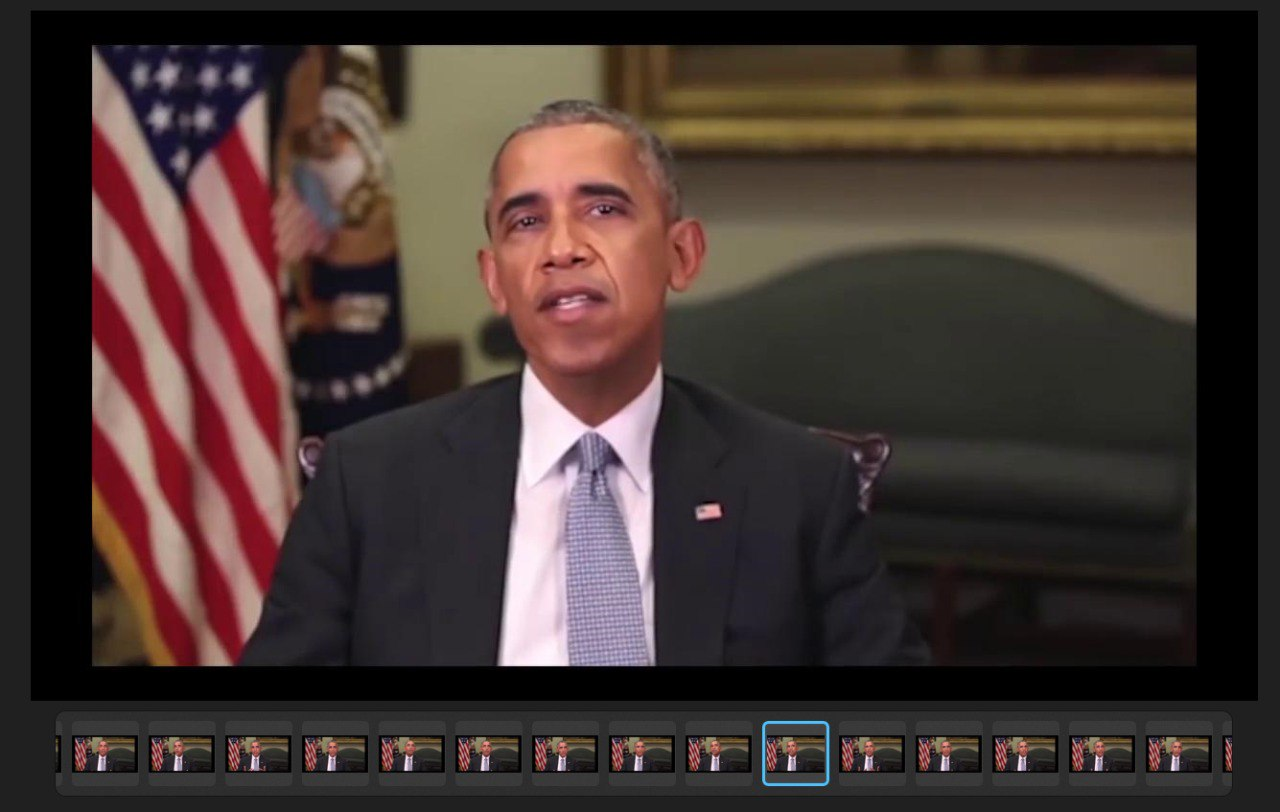
\includegraphics[width= 5in ]{img/frameSelected.jpg}
    \caption{Seleting required frames}
\end{figure}


\subsubsection{Annotation and Labeling}
Each image was labeled as either "real" or "deepfake." Annotations were done manually to ensure accurate labeling for training and evaluation.

\newpage